\documentclass[11pt,a4paper]{article}

\setlength {\marginparwidth }{2cm}

\usepackage[margin=2.5cm]{geometry}
\usepackage{todonotes}
\usepackage[automake]{glossaries}
\usepackage{graphicx}
\usepackage{microtype}
\usepackage{listings}
\usepackage{color}
\usepackage{amssymb,amsmath}
\usepackage{mathpazo}
\usepackage{accents}
\usepackage{longtable,booktabs}
\usepackage{dcolumn}
\usepackage{pgf}
\usetikzlibrary{shapes.geometric}
\usetikzlibrary{matrix}
\usepackage{natbib}
\usepackage{hyperref}
\usepackage[capitalise,noabbrev,nameinlink]{cleveref}
\hypersetup{
  pdftitle={Input-Endorsers Solution Primer},
  pdfborder={0 0 0},
  breaklinks=true
}
\graphicspath{ {./images/} }

\definecolor{dkgreen}{rgb}{0,0.6,0}
\definecolor{gray}{rgb}{0.5,0.5,0.5}
\definecolor{pink}{rgb}{0.92,0.2,0.86}

\lstset{frame=tb,
  language=Haskell,
  aboveskip=3mm,
  belowskip=3mm,
  showstringspaces=false,
  columns=flexible,
  basicstyle={\ttfamily},
  numbers=none,
  numberstyle=\tiny\color{pink},
  keywordstyle=\color{pink},
  commentstyle=\color{pink},
  stringstyle=\color{pink},
  breaklines=true,
  breakatwhitespace=true,
  tabsize=3
}

\DeclareMathOperator{\dom}{dom}
\newcommand\restrict[2]{\left.#1\right||_{#2}}
\newcommand\deltavar[1]{\accentset{\Delta}{#1}}

\makeglossaries
\newglossaryentry{rb}
{
    name={Ranking Block},
    description={a block which is responsible for transporting references to \glsplural{ib}}
}
\newglossaryentry{ib}
{
    name={Input Block},
    description={a block which is responsible for transporting transactions (or references to transactions)}
}
\newglossaryentry{tier}
{
    name={Tier},
    description={a grouping which attempts to classify priority of transport of \glsplural{ib}}
}
\newglossaryentry{tx}
{
    name={Transaction},
    description={an object representing UTxOs being spent (with or without a script context), to a destination address} 
}

\begin{document}

\title {Input-Endorsers Solution Primer \\
       {\large \sc An IOHK discussion paper}}
\date  {Version 0.1, 23rd June 2022}
\author{John Woods         \\ {\small \texttt{john.woods@iohk.io}} \\
                              {\small \texttt{john@postquantum.dev}} \\
}

\maketitle

\section{Purpose}
The purpose of this document is to provide a macroscopic view of the current state of 
research, a potential architectural design, and highlight possible design pitfalls 
with regard to the upcoming \emph{Input-Endorsers} protocol enhancement. \\ 

The goal of the Input-Endorsers enhancement is to minimize under-utilization of Cardano's system resources.
As of writing, approximately 25\% ($5$ seconds out of each $20$ second period) are currently being used to process
transactions. The remaining 75\% of the time is spent idle, filling mempool, or dedicated to other tasks
which do not contribute to the bandwidth of the Cardano network. \\

Thus, the goal with the introduction of Input-Endorsers is to achieve a higher transaction throughput
by utilizing resources more efficiently, and more effectively. This change (which will touch the three 
major system components: Consensus, Ledger \& Network) will also pave the way for the introduction of tiered
pricing, which is also discussed herein. \\

This document will look at hypothetical requirements (motivation/business caes), highlight a potential high-level
architecture, and finally, shine a light on some potential "footguns" which the implementation should consider. 
The target audience for this document is Engineering, and it should be considered a disambiguation paper 
rather than a design document. As of writing, Research on Input-Endorsers is still ongoing, thus, design 
decisions are still in flux.
\pagebreak

\tableofcontents

\pagebreak

\section{Acknowledgements}
The ideas presented herein are inspired by and based on discussions with
people from the research and engineering groups, specifically: Aggelos Kiayias, 
Giorgos Panagiotakos, Matthias Fitzi, Sandro Coretti, Philip Lazos, Duncan Coutts,
Neil Davies, Benjamin Beckmann \& Vitor Silva.

\pagebreak

\section{Context}
Input-Endorsers are a major enhancement to the Cardano consensus protocol, Ouroboros.
Input-Endorsers decouple consensus \& transaction diffusion. Input-Endorsers represent 
Cardano's next-generation layer 1 scaling technology. \\ \\
It's recognized that Cardano's resources are currently under-utilized:

\begin{itemize}
  \item Less than 25\% of time is spent creating and transmitting blocks/transactions.
  \item More than 75\% of time is spent idle, waiting for a new block, or filling mempool.
\end{itemize}

\begin{figure}[ht]
  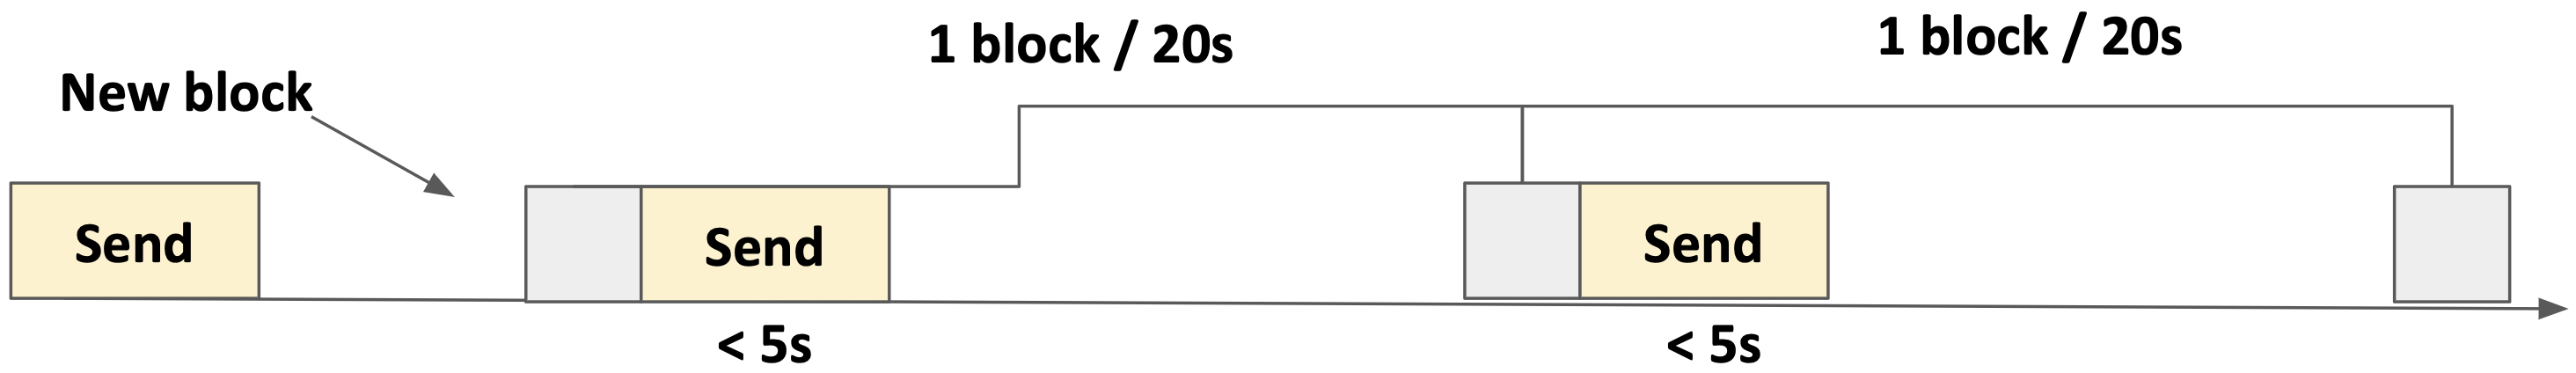
\includegraphics[width=\linewidth]{current_usage.png}
  \caption{current resource utilization}
  \label{fig:current utilization}
\end{figure}

In order to achieve higher throughput we must utilize resources more effectively.
The key insight with Input-Endorsers is the realization that with a single block
type, each block is responsible for \emph{both} transaction propagation (as transactions are a 
given block's payload) \emph{and} for consensus. However, if we introduce a scheme which 
\emph{decouples} consensus from transaction propagation, achieved by employing \emph{two} 
different block types, we can then reduce low resource utilization, and achieve higher
transaction throughput. \\

As we cannot naïvely increase block production to increase throughput (due to the danger of increased 
forks/height battles), instead consider the following scheme, which depicts a construction which may 
be used to achieve a more effective utilization of the Cardano network's resources:

\begin{figure}[ht]
  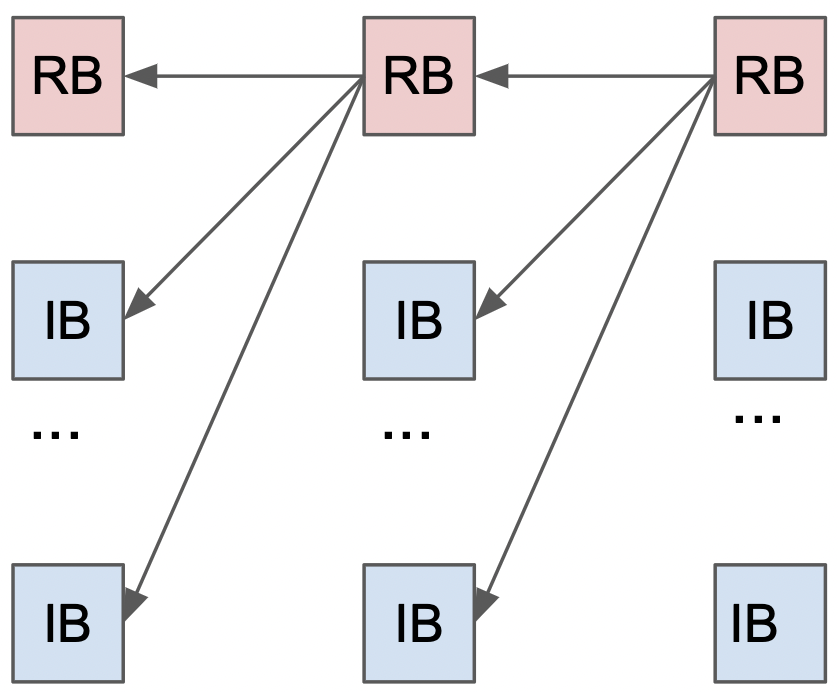
\includegraphics[width=0.4\textwidth]{ie_structure.png}
  \centering
  \caption{proposed block re-structure}
  \label{fig:proposed re-structure}
\end{figure}

\pagebreak

\textbf{Input-Endorsers} introduces \emph{two} categories of blocks:
\begin{itemize}
  \item \emph{\glsplural{rb}}: responsible for consensus. 
    \subitem \textbf{Payload}: \gls{ib} references.
  \item \emph{\glsplural{ib}}: responsible for transaction propagation.
    \subitem \textbf{Payload}: \gls{tx} references.
\end{itemize}

\textbf{\glsplural{rb}} will use reference semantics to reference \glsplural{ib}, \glsplural{rb} will still employ
the "longest chain" rule. They will be solely responsible for consensus and shall have a "low"
production rate, which is expected to be similar to our current block production rate, approximately 
one block every $20$ seconds. \glsplural{rb} will have low resource utilization. \\

\textbf{\glsplural{ib}} \emph{should} \emph{may} also use reference semantics, which is discussed further herein 
(\emph{note: in preliminary research artefacts \glsplural{ib} employed value semantics rather than reference 
semantics}) \glsplural{ib} will carry a payload of transaction references, and will be solely responsible for 
propagation and ordering of transactions. The actual transaction data may be propagated separately. 
This approach is being considered to:

\begin{itemize}
  \item Reduce transmission of duplicate data over the network graph.
  \item Reduce the intersection size (overlap) of \glsplural{ib}.
\end{itemize}

Both of these topics are discussed further herein. \glsplural{ib} will have a "high" production rate, which is expected 
to yield a significant increase in throughput, thus: \\

\begin{itemize}
  \item \emph{\glsplural{rb} will order (serialize) \glsplural{ib}.} 
  \item \emph{\glsplural{ib} will order transactions.} \\
\end{itemize}

The scheme described above may be visualized in a timeline as:

\begin{figure}[ht]
  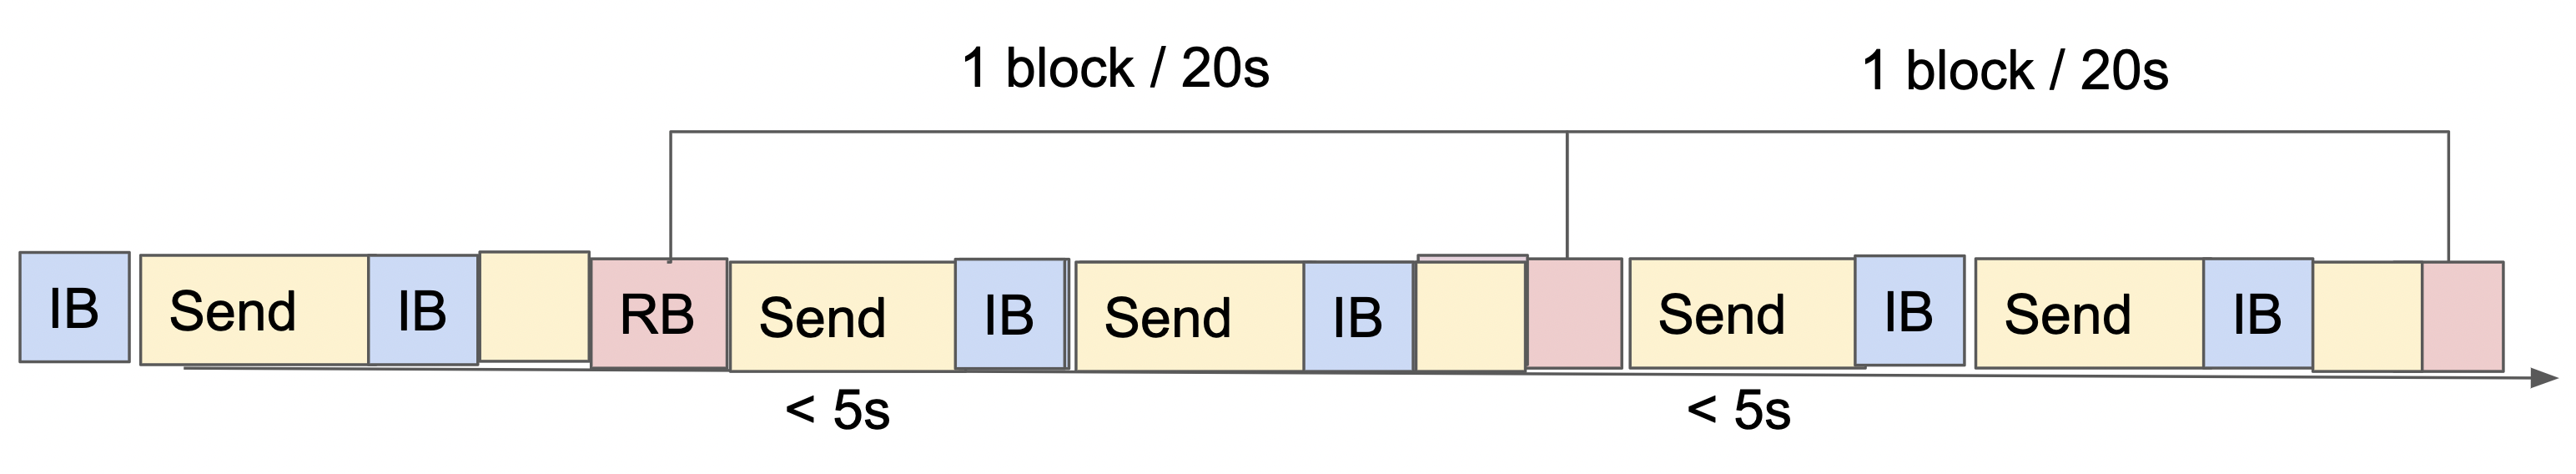
\includegraphics[width=\linewidth]{proposed_usage.png}
  \caption{proposed resource utilization}
  \label{fig:proposed utilization}
\end{figure}

\pagebreak

\section{Solution discussion}
Following is a high-level view into aspects of the technical architecture required for Input-Endorsers.
In this section we explore and discuss technical cornerstones of the design, some of which are a radical
departure from our current implementation of Ouroboros, and indeed the Ledger rules. \\ 

Additionally, it is important to note that the following should be considered a hypothetical approach, 
not a canonical design document. Ultimately our goal is to deliver on the functional and non-functional 
requirements, without adding unnecessary complexity to the system components. \\

Input-Endorsers provides high throughput by design. Thus, the engineering challenge effectively changes from 
\emph{"How do we increase the throughput of the system?"} to \emph{"How do we maximize efficacy and eliminate 
redundant data propagation?"} \\

In following sections we will discuss technical approaches which may be used to solve this challenge.

\subsection{VRF Usage}
Both \glsplural{ib} \& \glsplural{rb} will be produced using the same VRF (verifiable random function) mechanism 
as per the current implementation of Ouroboros. That is, block producers will be \emph{selected} using a VRF. 
Both \glsplural{ib} and \glsplural{rb} production will have separate VRF calls, tuned by a parameter $\mathcal{F}$ to 
ensure optimal pacing for both block types. Therefore, the schedule of block production for \glsplural{ib} will be 
significantly higher than that for \glsplural{rb}. \\
Having two VRF functions with varying rates will also yield a more egalitarian distribution of rewards. 
SPOs which are currently unlikely to be selected for \gls{rb} production due to their stake set size will be more 
likely to qualify for \gls{ib} production, given their frequency.

\subsection{Mempool Design}
Mempool will also see significant change, though importantly it will maintain a \emph{FIFO} structure.
With the current implementation of the node there is a single Mempool which is responsible for
holding disseminated \emph{unprocessed} transactions. With Input-Endorsers, there will be two Mempools.

\begin{enumerate}
  \item A transaction Mempool (inbound Mempool which holds unprocessed transactions which were received either from 
        peers, or submitted locally).
  \item An \gls{ib} Mempool (outbound Mempool which holds \glsplural{ib} which are to be propagated to downstream 
        peers).
\end{enumerate} 

\ \\
Let us consider the following requirements which should influence our Mempool design:

\begin{itemize}
  \item Transactions should be processed quickly, with as little duplicate processing/data transmission as possible.
  \item SPO resource usage should be bounded (bounded resource will mitigate DDoS attack vectors).
  \item Transactions should have linear consistency (successive transactions sent from the same source should be 
        processed in chronological order).
\end{itemize}
\todo{further discussion of mempool design}


\subsection{"Colouring"}
With Input-Endorsers transaction processing throughput will be increased significantly. As outlined herein, this is the
primary benefit of employing two different block types (\glsplural{ib} \& \glsplural{rb}).
SPOs will create both \glsplural{ib} \& \glsplural{rb} as defined by the VRF schedule. One of the main challenges we 
face due to \glsplural{ib} high production rate is reduction of duplicate being transmitted over the network graph.
As each SPOs mempool naturally contains a similar set of unprocessed transactions, and given the high block production 
rate of \glsplural{ib}, we would expect to see a significant proportion of disparately produced \glsplural{ib} share 
a large intersection of their transaction sets. \\ The larger this intersection the lower the efficacy of the system.\\

In order to maximise throughput with Input-Endorsers it's important to engineer a mechanism so that SPOs select
transactions to include in \glsplural{ib} in a uniform distributed manner. Selection of transactions in a deterministic,
uniformly distributed random manner will provide an approach to minimize the intersection of two disparately produced 
\glsplural{ib}.


\subsection{Blockchain Structure}
Assumptions we had with regard to the blockchain structure will need to be reevaluated in the context of 
Input-Endorsers. Specifically, with Praos (and its single block type), one could previously reason that transactions 
in a given block in the chainDB (both immutable \& volatile portions) were linearly consistent. \\ 

That is, two discrete blocks would never contain transactions that attempted to spend the same UTxOs. This was due 
to the fact that chain extension, by definition, would only occur if a transaction spent UTxOs which were part of the 
current UTxO set. Of course, this set is calculated by applying the Ledger rules to all previous blocks in the 
chainDB.\\

Thus is was impossible to enter an inconsistent state where two discrete blocks contained transactions which 
contradicted each other, by spending the same UTxOs. \\

The above description of linear consistency is not applicable in the context of Input-Endorsers. Given the nature of 
transaction propagation with Input-Endorsers, transactions are carried as the payload of \glsplural{ib}. \glsplural{ib}
have, by design, a high rate of block production and are issued in parallel by multiple SPOs. Additionally, 
\glsplural{ib} though ordered by ranking blocks, may arrive out of order, or be delayed. This behaviour results in a 
chain which must handle branching and merging. This is something Praos did not have to consider. \\

In short, with Input-Endorsers, Ledger must be adjusted so that it can validate a given \gls{ib}, even when it may 
contain a transaction (or transactions), which attempt to spend UTxOs which are no longer part of the current UTxO set.
In such a case, Ledger should interpret the \gls{ib}, executing validation checks, but ignoring any subset of the 
transaction set contained by the \gls{ib} which attempts to include spent UTxOs. \\

\emph{This parallelism and need to handle inconsistency is an artefact of the concurrency gain provided by 
Input-Endorsers.}


\subsection{Attacks/Fragility}
\todo{a section on ensuring we do not permit unbounded work for good actors}

\subsection{Tiered Fees}
\todo{a section on how tiered fees might integrate with Input-Endorsers/Mempool}

\pagebreak

\section{Conclusion}
Input-Endorsers will provide a significant increase in transaction throughput and transaction processing time for 
Cardano's L1. Whilst still in active research the technology apears compelling. The aforementioned notwithstanding, 
definition of a robust, scalable and secure solution architecture, and delivery of a high quality, production ready 
implementation will require a non-trivial engineering effort.

The next stages in bringing Input-Endorsers to market are:

\begin{enumerate}
  \item Align with Product to define requirements for the technology, including a business case for the effort.
  \item Await research outputs, which must be consumed and in-turn fuel construction of a full solution 
        design/architecture
  \item Provide hand-over of the validated architecture (after DEDA), to the engineering team for assimilation into 
        their backlog. 
\end{enumerate}

\pagebreak

\printglossaries

\end{document}